\subsection*{1.1}
  % Implement  the  common-source  MOS  amplifier  shown  below.  
  The circuit in figure 1 was implemented in NI Multisim.
    \begin{figure}[h!]
        \centering
        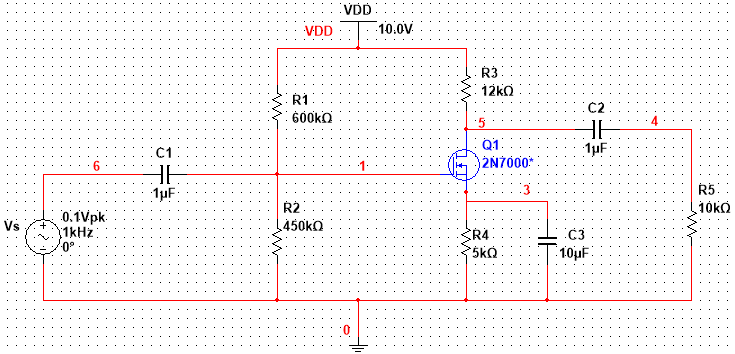
\includegraphics[width=6cm]{fig1-1-multisim.png}
        \captionof{figure}{The CS MOS amplifier implemented in Task 1.1}
    \end{figure} 
  The  transistor  model was modified to look as follows:\\
  Cgs  2 3 20E-12\\ 
  Cgd 1 2 10E-12\\
  M1 1 2 3 3 MOST1 W=500u L=2u\\
  .MODEL MOST1 NMOS(Level=3 Kp=20u W=500u L=2u Rs=20m Vto=2 Rd=1.186)\\\\

  The following parameters were used: kn =  20  $\mu$A/V2,  W/L =  250,  VT =  2  V,  Cgs =  20  pF, Cgd = 10 pF\\

\subsection*{1.2}
  % Using  the  above  parameters  (here:  kn =  20  µA/V2,  W/L =  250,  VT =  2  V,  Cgs =  20  pF,
  % Cgd = 10 pF) perform the theoretical analysis of the circuit to find the voltage gain, input
  % resistance, output resistance, as well as to estimate the lower and upper 3dB frequencies.

  A theoretical analysis of the circuit in figure 1 was performed to find the voltage gain, input resistance, output resistance, as well as to estimate the lower and upper 3dB frequencies.\\\\

  To find the voltage gain the DC current, I$_D$, was found to be 379$\mu$A and used to calculate g$_m$ = $\frac{1}{513.5 \omega}$. Using the small signal t-model the midband gain was found to be $\frac{v_o}{v_i} = |-10.615| \frac{V}{V} = 20.518 dB$.\\\\

  The lower and upper 3dB frequencies were found doing a low and high frequency analysis of the circuit. Capacitors C$_1$1, C$_2$ and C$_3$ are much larger than capacitors C$_{gs}$ and C$_{gd}$ so for the low frequency analysis C$_{gs}$ and C$_{gd}$ can be neglected and vice versa.\\

  Calculations from the high frequency analysis using a small signal hybrid-pi model show that f$_{H 3dB} = 2.918$MHz\\

  Calculations from the low frequency analysis using a small signal T model show that f$_{L 3dB} = 34.18$Hz\\

  The input resistance of the circuit, R$_{in}$, is the parallell connection of R$_{G1}$ and R$_{G2}$, R$_{in}$ = $R_{G1}||R_{G2}$ = 257k$\omega$.\\
  The output resitance of the circuti, R$_{out}$, is the drain resistance, R$_D$ = 12k$\omega$.\\\\

  All calculations can be seen in Appendix 1.

\subsection*{1.3}
  % Determine the values of the same parameters by simulation. Note that in order to obtain
  % some  of  the  parameters  certain  changes  in  the  circuit  diagram  and/or  introducing  some
  % auxiliary elements may be necessary. 

  A simulation was done for the circuit in figure 1 to find the voltage gain, input resistance, output resistance, as well as to estimate the lower and upper 3dB frequencies.\\\\

  The drain current was found using a DC operating point analysis and the results show that I$_D$ = 379.244$\mu$A as seen in figure 2. The voltage at the top node is positive so the current is flowing downward from this perspective.\\

  \begin{figure}[h!]
        \centering
        \includegraphics[width=6cm]{fig1-3-current.png}
        \captionof{figure}{DC operating point analysis used to find the drain current}
  \end{figure}

  An AC analysis was used to find the gain, f$_{L 3dB}$ and f$_{H 3dB}$. From the results of this analysis seen in figure 3 and 4, the gain is $\frac{v_o}{v_i} = 20.521 dB = 10.618 \frac{V}{V}$, f$_{L 3dB} = 35.592$ Hz and f$_{H 3dB} = 2.953$ MHz.\\

  \begin{figure}[h!]
        \centering
        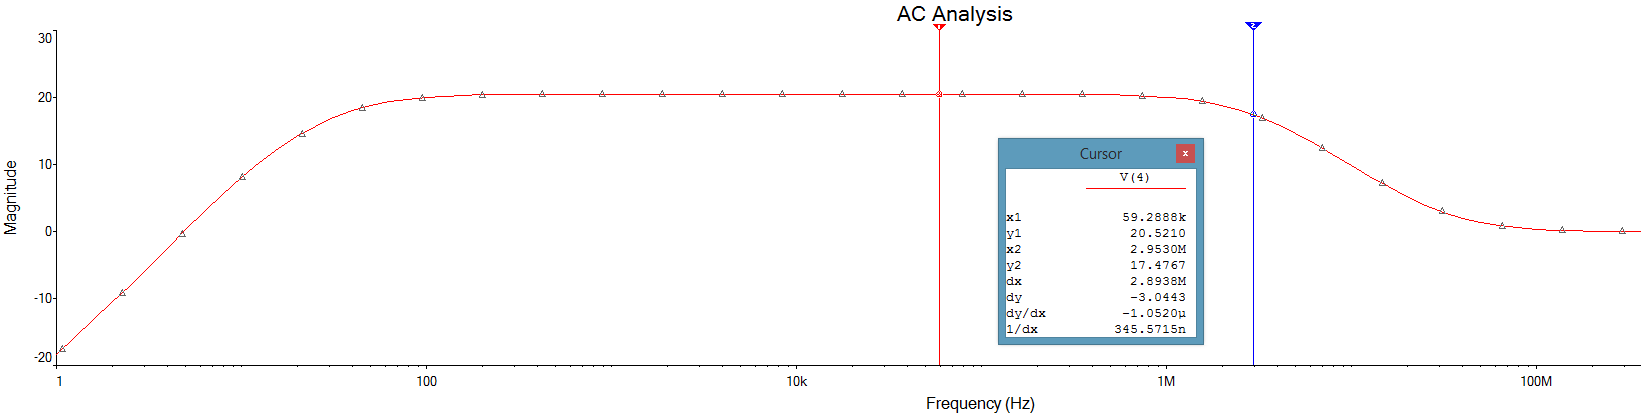
\includegraphics[width=6cm]{fig1-3-fh.png}
        \captionof{figure}{The AC analysis used to find the gain and f$_{H 3dB}$}
  \end{figure}

  \begin{figure}[h!]
        \centering
        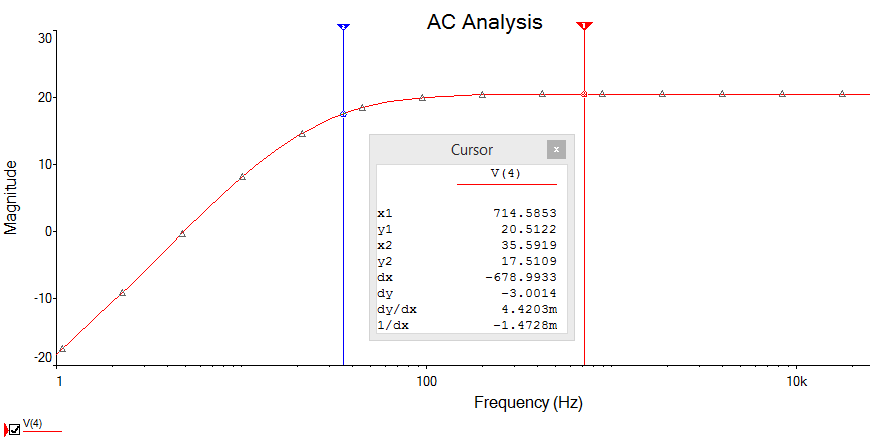
\includegraphics[width=6cm]{fig1-3-fl.png}
        \captionof{figure}{The AC analysis used to find f$_{L 3dB}$}
  \end{figure}

  Simulations to find R in and R out.....\\\\\\




\subsection*{1.4}
  % Compare the parameters obtained by simulation with those obtained from the theory and
  % comment upon possible differences.
  